%% Verze pro jednostranný tisk:
%\documentclass[11pt,a4paper]{report}
%\usepackage[top=25mm,bottom=25mm,right=25mm,left=30mm,head=12.5mm,foot=12.5mm]{geometry}
%\let\openright=\clearpage

%% Pokud tiskneme oboustranně:
\documentclass[11pt,a4paper,openany]{report}

%% - - - - - - - - - - - - - - - - - - - -  %%
 
\setlength{\arrayrulewidth}{0.5mm}
\setlength{\tabcolsep}{18pt}
\renewcommand{\arraystretch}{2.5}

\usepackage{makecell}

\renewcommand\theadalign{bc}
\renewcommand\theadfont{\bfseries}
\renewcommand\theadgape{\Gape[4pt]}
\renewcommand\cellgape{\Gape[4pt]}

%% - - - - - - - - - - - - - - - - - - - -  %%

%% Definice různých užitečných maker (viz popis uvnitř souboru)
%%% Tento soubor obsahuje definice různých užitečných maker a prostředí %%%
%%% Další makra připisujte sem, ať nepřekáží v ostatních souborech.     %%%

\usepackage[a-2u]{pdfx}     % výsledné PDF bude ve standardu PDF/A-2u
\usepackage[top=25mm,bottom=25mm,right=25mm,left=30mm,head=12.5mm,foot=12.5mm]{geometry}
\let\openright=\cleardoublepage
 
%%% Nastavení pro použití samostatné bibliografické databáze.
\usepackage[
   autocite = superscript,
   backend  = biber,
   style    = iso-numeric,
   language = czech,
   sorting  = nty,
   bibencoding = UTF8
]{biblatex}
\addbibresource{law.bib}
\addbibresource{literatura.bib}

\DeclareCiteCommand{\supercite}[\mkbibsuperscript]
  {\iffieldundef{prenote}
     {}
     {\BibliographyWarning{Ignoring prenote argument}}%
   \iffieldundef{postnote}
     {}
     {\BibliographyWarning{Ignoring postnote argument}}}
  {\usebibmacro{citeindex}%
   \bibopenbracket\usebibmacro{cite}\bibclosebracket}
  {\supercitedelim}
  {}
  
\let\cite\supercite

\usepackage[justification=centering]{caption} % or e.g. [format=hang]

\usepackage{chngcntr}
\counterwithout{figure}{chapter}
\counterwithout{table}{chapter}

%% TODOs
\setlength{\marginparwidth}{2cm}
\usepackage[colorinlistoftodos,prependcaption,textsize=tiny]{todonotes}

%% Přepneme na českou sazbu, fonty Latin Modern a kódování češtiny
\usepackage[czech]{babel}
\usepackage{lmodern}
\usepackage[T1]{fontenc}
\usepackage{textcomp}
\usepackage[utf8]{inputenc}
\usepackage{csquotes}

%%% Další užitečné balíčky (jsou součástí běžných distribucí LaTeXu)
\usepackage{amsmath}        % rozšíření pro sazbu matematiky
\usepackage{amsfonts}       % matematické fonty
\usepackage{amsthm}         % sazba vět, definic apod.
\usepackage{bm}             % tučné symboly (příkaz \bm)
\usepackage{graphicx}       % vkládání obrázků
\usepackage{fancyvrb}       % vylepšené prostředí pro strojové písmo
\usepackage{fancyhdr}       % prostředí pohodlnější nastavení hlavy a paty stránek
\usepackage{icomma}         % inteligetní čárka v matematickém módu
\usepackage{dcolumn}        % lepší zarovnání sloupců v tabulkách
\usepackage{booktabs}       % lepší vodorovné linky v tabulkách
\makeatletter
\@ifpackageloaded{xcolor}{
   \@ifpackagewith{xcolor}{usenames}{}{\PassOptionsToPackage{usenames}{xcolor}}
  }{\usepackage[usenames]{xcolor}} % barevná sazba
\makeatother
\usepackage{multicol}       % práce s více sloupci na stránce
\usepackage{caption}
\usepackage{enumitem}
\setlist[itemize]{noitemsep, topsep=0pt, partopsep=0pt}
\setlist[enumerate]{noitemsep, topsep=0pt, partopsep=0pt}
\setlist[description]{noitemsep, topsep=0pt, partopsep=0pt}

\usepackage{float}
\usepackage{numprint}

\usepackage[acronym,nopostdot,toc]{glossaries}
\usepackage[bottom]{footmisc}

\usepackage{tabu}
\usepackage{longtable}

\usepackage{pdfpages}
\usepackage{tocloft}

\setlength\cftparskip{0pt}
\setlength\cftbeforechapskip{1.5ex}
\setlength\cftfigindent{0pt}
\setlength\cfttabindent{0pt}
\setlength\cftbeforeloftitleskip{0pt}
\setlength\cftbeforelottitleskip{0pt}
\setlength\cftbeforetoctitleskip{0pt}
\renewcommand{\cftlottitlefont}{\Huge\bfseries\sffamily}
\renewcommand{\cftloftitlefont}{\Huge\bfseries\sffamily}
\renewcommand{\cfttoctitlefont}{\Huge\bfseries\sffamily}

% vyznaceni odstavcu
\parindent=0pt
\parskip=11pt

% zakaz vdov a sirotku - jednoradkovych pocatku ci koncu odstavcu na prechodu mezi strankami
\clubpenalty=1000
\widowpenalty=1000
\displaywidowpenalty=1000

% nastaveni radkovani
\renewcommand{\baselinestretch}{1.20}

% nastaveni pro nadpisy - tucne a bezpatkove
\usepackage{sectsty}    
\allsectionsfont{\sffamily}

% nastavení hlavy a paty stránek
\fancyhf{}
\fancyhead[R]{\rightmark}
\fancyfoot[R]{\thepage}
\renewcommand{\footrulewidth}{.5pt}
\fancypagestyle{plain}{%
\fancyhf{} % clear all header and footer fields
\fancyfoot[R]{\thepage}
\renewcommand{\headrulewidth}{0pt}
\renewcommand{\footrulewidth}{0.5pt}}

% Tato makra přesvědčují mírně ošklivým trikem LaTeX, aby hlavičky kapitol
% sázel příčetněji a nevynechával nad nimi spoustu místa. Směle ignorujte.
\makeatletter
\def\@makechapterhead#1{
  {\parindent \z@ \raggedright \sffamily
   \Huge\bfseries \thechapter. #1
   \par\nobreak
   \vskip 20\p@
}}
\def\@makeschapterhead#1{
  {\parindent \z@ \raggedright \sffamily
   \Huge\bfseries #1
   \par\nobreak
   \vskip 20\p@
}}
\makeatother

% aquote pro blokovou citaci s autorem vpravo dole
\def\signed #1{{\leavevmode\unskip\nobreak\hfil\penalty50\hskip2em
  \hbox{}\nobreak\hfil(#1)%
  \parfillskip=0pt \finalhyphendemerits=0 \endgraf}}

\newsavebox\mybox
\newenvironment{aquote}[1]
  {\savebox\mybox{#1}\begin{quote}}
  {\signed{\usebox\mybox}\end{quote}}

% Trochu volnější nastavení dělení slov, než je default.
\lefthyphenmin=2
\righthyphenmin=2

% Zapne černé "slimáky" na koncích řádků, které přetekly, abychom si
% jich lépe všimli.
\overfullrule=1mm

%% Balíček hyperref, kterým jdou vyrábět klikací odkazy v PDF,
%% ale hlavně ho používáme k uložení metadat do PDF (včetně obsahu).
%% Většinu nastavítek přednastaví balíček pdfx.
\hypersetup{unicode}
\hypersetup{breaklinks=true}
\hypersetup{hidelinks}

%%% Prostředí pro sazbu kódu, případně vstupu/výstupu počítačových
%%% programů. (Vyžaduje balíček fancyvrb -- fancy verbatim.)

\DefineVerbatimEnvironment{code}{Verbatim}{fontsize=\small, frame=single}


%%% Useful law-related macros
\usepackage{pgfkeys}
\pgfkeys{
    /paragraph/.is family, /paragraph,
    default/.style = {z = 90, rok = 2012, odst = 0},
    z/.estore in = \paragraphZakon,
    rok/.estore in = \paragraphRok,
    odst/.estore in = \paragraphOdst,
}

\newcommand{\lawp}[2][]{
    \pgfkeys{/paragraph, default, #1}%
    \ifthenelse{\paragraphOdst =0}{%
        \href{https://www.zakonyprolidi.cz/cs/\paragraphRok-\paragraphZakon\#p#2}
        {\textbf{§~#2 zákona č. \paragraphZakon/\paragraphRok~Sb.}}\cite{\paragraphZakon/\paragraphRok p#2}}{%
        \href{https://www.zakonyprolidi.cz/cs/\paragraphRok-\paragraphZakon\#p#2-\paragraphOdst}
        {\textbf{§~#2 odst. \paragraphOdst~zákona č. \paragraphZakon/\paragraphRok~Sb.}}\cite{\paragraphZakon/\paragraphRok p#2-\paragraphOdst}}%
}


%%% Údaje o práci
% Název práce v jazyce práce (přesně podle zadání)
\def\NazevPrace{Generace X vs. Generace Y --- jak se chovají jako zákazníci?}

% Typ práce
\def\TypPrace{SEMINÁRNÍ PRÁCE}
%\def\TypPrace{DIPLOMOVÁ PRÁCE}


% Jméno autora
\def\AutorPrace{Bc. Marek Čermák}

% Rok odevzdání. měsíc (slovně)
\def\DatumOdevzdani{Listopad 2019}

% Vedoucí práce: Jméno a příjmení s~tituly
\def\Vedouci{Mgr. Tomáš Zdražil}

% Studijní program a obor
% \def\StudijniProgram{studijní program}
% \def\StudijniObor{studijní obor}

% Text čestného prohlášení pro MUŽE pro tuto prácí
\def\Prohlaseni{Prohlašuji, že jsem tuto práci \textit{\NazevPrace} vypracoval samostatně za použití v práci uvedených pramenů a literatury.}
% Text čestného prohlášení pro MUŽE pro bakalářskou prácí
% \def\Prohlaseni{Prohlašuji, že jsem bakalářskou práci \textit{\NazevPrace} vypracoval samostatně za použití v práci uvedených pramenů a literatury.}
% Text čestného prohlášení pro MUŽE pro diplomovou prácí
%\def\Prohlaseni{Prohlašuji, že jsem diplomovou práci \textit{\NazevPrace} vypracoval samostatně za použití v práci uvedených pramenů a literatury.}
% Text čestného prohlášení pro ŽENY pro bakalářskou prácí
%\def\Prohlaseni{Prohlašuji, že jsem bakalářskou práci \textit{\NazevPrace} vypracovala samostatně za použití v práci uvedených pramenů a literatury.}
% Text čestného prohlášení pro ŽENY pro diplomovou prácí
%\def\Prohlaseni{Prohlašuji, že jsem diplomovou práci \textit{\NazevPrace} vypracovala samostatně za použití v práci uvedených pramenů a literatury.}

% Nepovinné poděkování (vedoucímu práce, konzultantovi, tomu, kdo
% zapůjčil software, literaturu apod.)
\def\Podekovani{%
Poděkování.
}

% Abstrakt (doporučený rozsah cca 150-250 slov; nejedná se o zadání práce)
\def\Abstrakt{%
Abstrakt.
}
\def\AbstraktEN{%
Abstract.
}

% 3 až 5 klíčových slov (doporučeno)
\def\KlicovaSlova{klíčové slovo, další pojem, jiný důležitý termín, a ještě jeden}
\def\KlicovaSlovaEN{keyword, important term, another topic, and another one}

%% - - - - - - - - - - - - - - - - - - - -  %%

%% Zkratky
\makeglossaries
\newglossaryentry{noz}{type=\acronymtype, name=\makebox[2.5cm][l]{NOZ},      text={NOZ},      description=Občanský zákoník}
\newglossaryentry{zok}{type=\acronymtype, name=\makebox[2.5cm][l]{ZOK},      text={ZOK},      description=Zákon o obchodních společnostech a družstvech}
\newglossaryentry{ss} {type=\acronymtype, name=\makebox[2.5cm][l]{SS},       text={SS},       description=Společenská smlouva}
\newglossaryentry{vos}{type=\acronymtype, name=\makebox[2.5cm][l]{v. o. s.}, text={v. o. s.}, description=Veřejná obchodní společnost}
\newglossaryentry{sro}{type=\acronymtype, name=\makebox[2.5cm][l]{s. r. o},  text={s. r. o},  description=Společnost s ručením omezeným}
\newglossaryentry{ks} {type=\acronymtype, name=\makebox[2.5cm][l]{k. s.},    text={k. s.},    description=Komanditní společnost}
\newglossaryentry{as} {type=\acronymtype, name=\makebox[2.5cm][l]{a. s.},    text={a. s.},    description=Akciová společnost}

%% - - - - - - - - - - - - - - - - - - - -  %%

\begin{document}

%% Titulní strana a různé povinné informační strany
%%% Titulní strana práce a další povinné informační strany

%%% Titulní strana práce

\pagestyle{empty}
\hypersetup{pageanchor=false}

\begin{center}
\Huge\sffamily
Master of Business Administration\\
Executive Management Online

OBCHODNÍ PRÁVO


\vspace{\stretch{4}}
\bigskip


\includegraphics[width=.3\textwidth]{img/logo-cambschool.jpeg}

\vspace{\stretch{10}}

\bfseries\NazevPrace

\vspace{8mm}
\mdseries\TypPrace

\vspace{8mm}
\large
\begin{tabular}{rl}
\end{tabular}

\vspace{\stretch{10}}

\begin{tabular}{rl}
Autor: & \AutorPrace \\
\noalign{\vspace{1mm}}
Lektor: & \Vedouci \\
\end{tabular}

\vspace{6mm}
% Brno, \DatumOdevzdani
\end{center}


\openright

%%% Strana s čestným prohlášením k bakalářské práci

\thispagestyle{empty}
\hypersetup{pageanchor=true}
\pagestyle{plain}
\cleardoublepage
\section*{Prohlášení}
\noindent
\Prohlaseni

\vspace{2cm}
\noindent
V Praze dne
\hfill%
\begin{minipage}[t]{.5\textwidth}%
\begin{center}
\dotfill\\
Podpis studenta
\end{center}
\end{minipage}
\vspace{1cm}

% \newpage

%%% Poděkování
% \vspace*{\fill}
% \section*{Poděkování}
% \noindent
% \Podekovani
% \vspace{1cm}

% \newpage

%%% Povinná informační strana bakalářské práce
% \section*{Abstrakt}
% \noindent
% \Abstrakt
% \subsection*{Klíčová slova}
% \noindent
% \KlicovaSlova

% \newpage

% \bigskip\bigskip\bigskip
% \section*{Abstract}
% \noindent
% \AbstraktEN
% \subsection*{Keywords}
% \noindent
% \KlicovaSlovaEN


%%% Strana s automaticky generovaným obsahem bakalářské práce
\tableofcontents
\thispagestyle{empty}

%% Obrázky v bakalářské práci
\openright
\listoffigures

%%% Tabulky v bakalářské práci (opět nemusí být nutné uvádět)
\clearpage
\listoftables

%%% Použité zkratky v bakalářské práci (opět nemusí být nutné uvádět)
\setlength{\glsdescwidth}{0.7\textwidth}
\printglossary[type=\acronymtype, style=index, title=Seznam použitých zkratek]

\pagestyle{fancy}
\setcounter{tocdepth}{2}

%%% Jednotlivé kapitoly práce jsou pro přehlednost uloženy v samostatných souborech
\chapter*{Úvod}
\addcontentsline{toc}{chapter}{Úvod}


\chapter{Marketing}\label{ch:marketing}

Marketing je všeude kolem nás. Týká se nás více či méně, ať už si to uvědomujeme, nebo ne. V této kapitole uvedeme pojem \textbf{marketing} a seznámíme se s jeho účelem, hodnotami a procesem.

\section{Účel marketingu}

Jedna z nejstručnějších definic marketingu říká, že \textbf{marketing} je o naplňování potřeb se ziskem.\cite{kotler2007marketingmanagement} Marketing tak činí komplexní řadou aktivit, které zahrnují tvorbu výrobků a služeb, podporu jejich existence a vlastností a jejich fyzického zpřístupnění cílovým uživatelům -- distribuce.\cite{clemente2004slovnikmarketingu}
Tyto aktivity jsou známé jako tzv. \textbf{\uv{4P marketingu}} nebo také \textbf{\uv{merketingový mix}} (viz dále).

V zásadě můžeme také rozlišovat mezi \textbf{společenskou} a \textbf{manažerskou} definicí marketingu. Společenská definice chápe marketing jako společenský proces, ve kterém jsou hlavními aktéry jedinci a skupiny, kteří svobodně směňují, tj. nabízí a kupují, výrobky a služby. Manažerská definice naopak dosazuje za hlavního aktéra samotného prodejce a označuje marketing jako "umění prodeje výrobků"\cite{kotler2007marketingmanagement}.
Prodej výrobků jistě uměním je, nicméně může být pro některé překvapením, že nejdůležitější částí marketingu není prodej!

Jak uvádí Peter Drucker, přední teoretik managementu\cite{kotler2007marketingmanagement}:
\begin{aquote}{Peter Drucker}
\uv{Lze předpokládat, že vždy bude existovat potřeba něco prodávat. Cílem marketingu je však učinit prodávání čímsi nadbytečným. Cílem marketingu je poznat a pochopit zákazníka natolik dobře, aby mu výrobek, nebo služba padly jako šité na míru a prodávaly se samy. V ideálním případě by měl marketing vyústit v získání zákazníka ochotného nakupovat. Vše, čeho je pak zapotřebí, je učinit výrobek, či službu dostupnými.}
\end{aquote}

\section{4P marketingu}

Pojem \uv{marketingový mix}, známý také jako tzv. \uv{4P marketingu}, začal používat ve svých projevech prof. Neihl H. Borden a definoval jej v jedné ze svých publikací\cite{borden1964marketingmix} v roce 1949. V publikaci Borden říká, že tento pojem mu vnukl jeho spolupracovník -- prof. James Culliton. Ve své studii z roku 1948 Culliton definoval výkoného manažera jako umělce, který \uv{míchá ingredience} a který se \uv{někdy řídí receptem připraveným ostatními, jindy vymýšlí svůj vlastní. Někdy přihodí do receptu ingredienci, které je zrovna dostupná a jindy experimentuje s ingrediencemi, které nikdo nikdy nezkoušel.}

Marketingový mix tvoří čtyři kontrolovatelné proměnné, které společnost reguluje, aby efektivně prodávala výrobek. Jedná se o proměnné: \textbf{výrobek}, \textbf{cena}, \textbf{místo} a \textbf{reklama} (z anglického \textit{product}, \textit{price}, \textit{place}, \textit{promotion})\cite{clemente2004slovnikmarketingu}.
S nadsázkou lze o marketingu prohlásit, že se jedná pouze o to postavit správný produkt na správné místo za správnou cenu ve správný čas. Možná proto také hovoříme o marketingu jako o vědě --- je potřeba udělat spoustu věcí správně.


\subsection{Výrobek}
    
Výrobek je definován jako entita mající objektivní a subjektivní charakteristiky, které jsou manipulovány k maximu jeho přitažlivosti pro cílové zákazníky\cite{clemente2004slovnikmarketingu}. Výrobkem je tedy v podstatě jakékoli \textit{průmyslové} či \textit{spotřební zboží} vytvořené za účelem zisku.
Průmyslové zboží je zboží určeno primárně pro výrobu dalších výrobků. Patří sem například suroviny, zařízení nebo zpracovatelské materiály.
Spotřební zboží pak lze dále dělit na zboží \textit{dlouhodobé} a \textit{krátkodobé spotřeby} a \textit{balené} zboží.


\subsection{Cena}
Cena je jediným prvkem marketingového mixu, který společnosti \textbf{generuje výnosy}. Vztahuje se k stanovení nákladů na výrobek k maximálnímu prodeji a zvýšení image výrobku. Cena má nezanedbatelný vliv na představu spotřebitele o výrobku\cite{clemente2004slovnikmarketingu}.


\subsection{Místo}
Každý výrobek je potřeba někde skladovat a nějakým způsobem distribuovat (distribuce se týká i služeb) spotřebitelům. K tomu je potřeba vhodná \textit{taktika} a \textit{distribuční kanály}. Distribuce pak může být jak fyzického charakteru -- skladování a přeprava, tak virtuálně (např. zakoupení poukazu či subskripce). Kanály dělíme obecně na \textit{přímé} a \textit{nepřímé}:

\begin{itemize}
    \item přímé kanály -- zahrnují prodej přímo spotřebitelům
    \item nepřímé kanály -- spoléhají se na maloobchodníky, velkoobchodníky a jiné zprostředkovatele\footnote{Ačkoli je tato metoda dražší, společnosti mohou dosáhnout více zákazníků pomocí nepřímých kanálů, než pomocí ostatních distribučních postupů\cite["marketingový mix", s. 114]{clemente2004slovnikmarketingu}}
\end{itemize}

Speciální kombinací přímých a nepřímých kanálů pak vznikají tzv. \textit{mnohonásobné kanály}. Pracovníci marketingu si pak ale musí být vědomi potenciálními rivaly mezi kanály.


\subsection{Reklama}
Slovník marketingu definuje reklamu jako \uv{Marketingové a komunikační taktiky používané k uvědomování cílových spotřebitelů o charakteristikách, přínosech a dostupnosti výrobku.}\cite["reklama", s. 115]{clemente2004slovnikmarketingu} Obyčejně reklama samotná není jedinou formou propagace produktu. Dalšími způsoby může být osobní prodej a publicita nebo P.R (z anglického \uv{\textit{public relations}}).


\section{Vývoj marketingu}

I pro člověka neznalého marketingové teorie není příliš obtížně pozorovat změny na trhu\footnote{V tomto kontextu myšleno jako trh spotřebitele, tj. skupiny potenciálních kupujících}.
Za hlavní \uv{viníky} těchto změn lze označit dva faktory, které měly (a mají) majoritní dopad na vývoj ekonomiky a rovněž marketingu -- \textbf{technologie} a s ní související \textbf{globalizace}. Kotler ve své knize \textit{Chaotika}\cite[s. 14]{kotler2009chaotika} uvádí:

\begin{aquote}{zdroj: \textit{Chaotika}}
\uv{Svět je propojenější a vzájemně závislejší než kdykoli předtím. Globalizace a technologie jsou dvěma hlavními silami, které vedly k vytvoření provázané křehkosti ve světové ekonomice.}
\end{aquote}

V novém informačním věku je produkční úroveň přesnější, reklama cílenější a nabídka personalizovaná. Dostupnost zboží je technologickým pokrokem v dopravě a komunikaci prakticky neomezená a v mnoha případech téměř okamžitá. Internet se stává \textbf{novým prodejním kanálem}. Díky rostoucí otevřenosti a dostupnosti internetu jsou spotřebitelé informovanější, porovnání výrobků desítek dodavatelů je dnes otázkou několika kliknutí a portály se plní uživatelskými recenzemi, ať už pozitivními, či nikoli.
Moderní spotřebitelé hodnotí značku podle toho, jak moc se o ní mluví, jak moc je autentická a jedinečná a jaké v emoce značka vyvolává. Chtějí se se značkou \textit{ztotožnit}.\cite{bergh2012coolznacky}
Tyto a další důvody vedou také k přesunu moci do rukou zákazníků --- slovní spojení \uv{náš zákazník, náš pán} tak v posledních letech dosahuje dosud nevídaných rozměrů --- a zákazníci tak očekávají stále lepší služby, vyšší kvalitu a pohodlí a individuální přístup.

\subsection{Holistický marketing}

Společnosti tak potřebují nový způsob myšlení o tom, jak působit a soupeřit v novém marketingovém prostředí. Touto novou koncepcí je tzv. \textit{holistický merketing}.
\uv{\textbf{Holistické marketingové pojetí} je postaveno na vývoji, designu a plnění marketingových programů, procesů a aktivit beroucích v úvahu jejich šíři a vzájemnou propojenost.}\cite{kotler2007marketingmanagement} Holistický marketing zavádí novou perspektivu, ve které \textbf{záleží na všem}. Jeho složky jsou shrnuty na obr. \ref{fig:slozky-holistickeho-marketingu}.

\begin{figure}[htbp!]
    \centering
    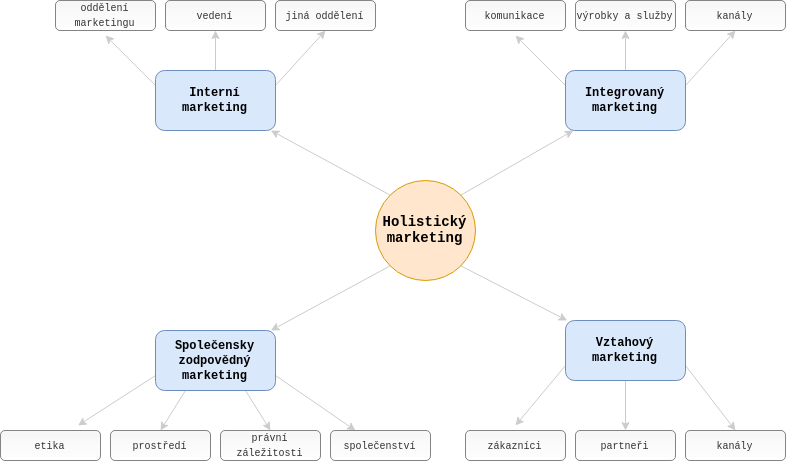
\includegraphics[width=.88\textwidth]{assets/slozky-holistickeho-marketingu.png}
    \caption[Složky holistického marketingu]{Složky holistického marketingu \\ Zdroj: Vlastní zpracování dle \textcite[s. 56]{kotler2007marketingmanagement}}
    \label{fig:slozky-holistickeho-marketingu}
\end{figure}

Je potřeba si uvědomit (a částečně se tak i uklidnit), že informační kvanta nejsou užitečná pouze a jen pro cílové spotřebitele, ale lze je s výhodou použít také pro marketingové účely.
\chapter{Historický přehled generací}

V průběhu 20. století a přelomu tisíciletí se vlivem světových událostí, technologickým rozkvětem a společenskými změnami utvářeli generace s charakteristickými rysy a rozdílným hodnotovým žebříčkem. Generací chápeme skupiny lidí se společnými znaky narozenou či vyrůstající v určitém časovém rozmezí. Sdílené prožitky tvarují a charakterizují osobnosti jedinců narozených v téže generaci.
Je důležité, aby si organizace byly vědomy těchto odlišností a rozdílných hodnotových žebříčků a jednali tak v jejich souladu a tvarovali se dynamicky s přicházejícími generacemi, které nahrazují ty předešlé. S novou pracovní silou přicházejí nové požadavky a potřeby.

V této kapitole budou uvedeny a stručně charakterizovány generace 20. století až po současnost. V další kapitole bude poté pozornost věnována generacím X a Y, které jsou předmětem této práce. Tyto generace momentálně zastávají největší část pracovního trhu\footnote{Dle časopisu Forbes je pouze Generace X v USA zodpovědná za více než třetinu státního příjmu.\cite{forbes2019generationX}}.

\section{Generace G.I.}
Tuto poválečnou generaci, nazývanou také jako \uv{The Greatest Generation}, jak ji nazval Tom Brokaw ve své stejnojmenné knize z roku 1998\cite{cnn2013americangenerationfacts}, tvoří skupina jedinců, kteří se narodili mezi lety 1900 až 1924. Tito lidé tedy zažili velkou depresi\footnote{Z anglického \textit{\uv{The Great Depression}}, byla největší ekonomickou recesí moderní historie a nejkatastrofičtější událostí 20. století\cite{investopedia2019thegreatdepression}} i druhou světovou válku.\\
V americkém pojetí je tato generace tzv. generací \textit{federace}. Její členové se zasloužili o vybudování Spojených Států, jak je známe dnes. Mezi nejznámnější patří tehdejší americký prezident J. F. Kennedy a další prezidenti: Richard M. Nixon, Gerald R. Ford, Ronald Reagan, Jimmy Carter, and George H.W. Bush. Děti této generace jsou známé jako generace \uv{baby boomers} (viz sekce \ref{sec:baby-boomers}).

\section{Tichá generace}
Označení \uv{tichá} odkazuje na konformistické tendence\cite{bergh2012coolznacky}, tj. přizpůsobování se převažujícím názorům a podřízení se společnosti a režimu nebo částečné potlačení vlastní identity. Vzhledem k časovému úseku, pro které je tato generace definována --- 1928 až 1945 --- tato konformita není příliš překvapivá. Tichá generace bývá označována za protiklad ke generaci baby boomu.


\section{Baby boomers}\label{sec:baby-boomers}
Označení generace baby boomu vychází z nárůstu porodnosti po skončení druhé světové války, který začal po jejím skončení a trval až do roku 1964 (komerční uvedení antikoncepce).\cite{bergh2012coolznacky} Tato generace zažívá technologický pokrok --- --- a je pro ni tedy charakteristická velká flexibilita a přizpůsobivost.
V současnosti tato generace zastává asi 20\rm \% celkové americké populace a zůstává tak zatím největší generací americké historie\cite{investopedia2019babyboomers} (toto se má změnit s příchodem mileniálů).


\section{Generace X}\label{sec:generace-x}
Podíváme-li se okolo sebe, pravděpodobně je okolo nás nějaký \textit{Gen X'er}, narozen v letech 1965 až 1979 (1981). Tato generace je často označována za generaci lenochů (slackers) a vyznačuje se lhostejností. Označení \textit{X} popularizovala kniha Douglase Couplanda \textit{Generace X}, ve které se generace nesnášející nálepky uvádí \uv{říkejte nám prostě X}.\cite{bergh2012coolznacky}
Členové této generace začínali kariéru v 90. letech, které se vyznačovaly ekonomickou recesí a snižováním stavů (a s výjimkou několika vzestupů tento stav alternoval prakticky až do roku 2010\cite{kotler2009chaotika}). Generace X ale převzala pracovní etiku a nasazení generace baby boomu a postupně začala utvářet ekonomiku (viz samostatná kapitola). Podle časopisu Forbes patří generace X k nejvzdělanějším --- 35\rm \% má vysokoškolský titul, v porovnání s 19\rm \% mileniálů.\cite{forbes2019generationX}


\section{Generace Y}\label{sec:generace-y}
Někdy označování jako \textit{mileniálové}, nebo také \textit{generace přelomu tisíciletí}, označuje populaci, jejíž představitelé se narodili v mezi roky 1980 a 1996. Zde jsou data poměrně flexibilní a někdy se uvádí za spodní hranici rok 1975, horním mezníkem pak dokonce rok 2005.\cite{rezlerova2007generacey} Generace baby boomu začala rodit později a jejich rodiče za ústřední princip považovali uznávání individuality.\cite{bergh2012coolznacky}

\section{Generace Z}\label{sec:generace-z}
Tato generace je první generací, která nezažila vyrůstání bez internetu, či nedostatku komodit. S počítačovou myší se naučili pracovat už v 18 měsících.\cite{bergh2012coolznacky} Technologie jsou pro ně samozřejmostí.
Jsou to děti generace X, kteří teprve vstupují na pracovní trh, proto o nich zatím mnoho nevíme. Je jisté, že tato generace bude technicky nejzdatnější a doposud nejdiverzitnější. Očekává se, že hlavním znakem této generace bude personalizace a kustomizace, tj. vše bude upraveno na míru.


\chapter{Generace X a Y jako spotřebitelé}

Výzkum centra Pew Research Center zjistil, že většina příslušníků každé generace je přesvědčena o své jedinečné, charakteristické identitě\cite[s. 22]{bergh2012coolznacky}.
Marketing se zabývá zjišťováním a naplňováním lidských a společenských potřeb.\cite[s. 43]{kotler2007marketingmanagement} Aby mohl být marketing vůbec úspěšný, je klíčové tuto identitu odhalit.
Jak ukazuje obrázek č. \ref{fig:us-population-by-generation}, generace X a Y souhrnně zastávají nejpočetnější zastoupení v současné populaci. Obě tyto generace mají nicméně jiné hodnoty, rozdílné životní priority, volný čas tráví odlišným způsobem, liší se ve formě komunikace mezi sebou atd. Z pohledu marketingu se tedy chovají jinak i jako spotřebitelé.
Cílem této kapitoly je podat ucelené srovnání těchto dvou skupin jako konzumentů a zjistit, jak se chovají jako zákazníci.

\medskip
\begin{figure}[htbp!]
    \centering
    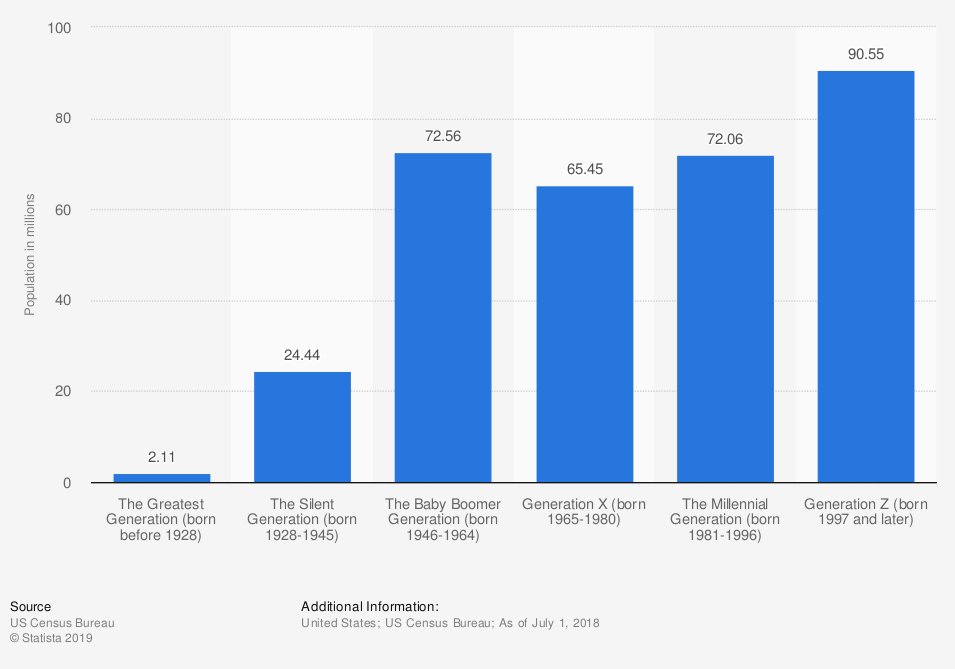
\includegraphics[width=.88\textwidth]{assets/us-population-by-generation.png}
    \caption[Populace US podle generace]{Populace US podle generace \\ Zdroj: Statista.com\protect\footnotemark~podle dat z US Census Bureau }
    \label{fig:us-population-by-generation}
\end{figure}

\footnotetext{Dostupné z: \url{https://www.statista.com/statistics/797321/us-population-by-generation/ }}

\section{Základní priority}
„Generace X byla svědkem kontrastu pracovního světa bez počítačů a příchodem technologií a digitálních inovací. Hodně porovnávají a dokážou ocenit rozsah a dopad těchto inovací, proto upřednostňují organizace, které „myslí dopředu“ a sledují aktuální technologické trendy,“ vysvětluje Ladislav Kučera v rozhovoru na téma \uv{pět generací zaměstnanců}.\cite{idnes2018generacezamestancu} Dále pak zdůrazňuje důraz generace X na rovnováhu mezi soukromým a pracovním životem - mají zodpovědnost za rodinu, děti. Tato generace je více než kterákoli jiná ochotna slevit ze svých mzdových nároků, jsou-li jí nabídnuty jiné výhody, jako je flexibilní pracovní doba, dovolená navíc, zdravotní péče a možnost pracovat z domova.

O generaci mileniálů pak personalista Ladislav Kučera prohlašuje: „Tato věková skupina je považována za zvlášť vytrvalou, ambiciózní, která se nebojí ve své kariéře trochu riskovat. Chce od svého zaměstnavatele slyšet konstruktivní zpětnou vazbu, očekává postup v rámci své role a společnosti“. (tamtéž)
Mileniálové nechtějí být omezováni hranicemi. Jsou si vědomi svých příležitostí a chtějí cestovat a získávat zahraniční zkušenosti.

\section{Média a sociální sítě}
Pro potřeby marketingu je nezbytně nutné šířit povědomí o značce a zvolit vhodné médium s ohledem na cílové zákazníky (reklama a místo jsou ostatně, jak bylo uvedeno, dvě ze čtyř P marketingu).
Přestože generace X se může jevit jako nihilistická a velmi individuálně zaměřená, podle časopisu Forbes má 81\rm \% této generace účet na Facebooku nebo jiné sociální síti\cite{forbes2019generationX} (údaj pro generaci Y sice neuvádějí, ale pravděpodobně bude přinejmenším stejně vysoké). Rozdíl ovšem je v tom, jak a jak často tyto sociální sítě využívají a jakou jim přikládají informační hodnotu.


\medskip
\begin{figure}[htbp!]
    \centering
    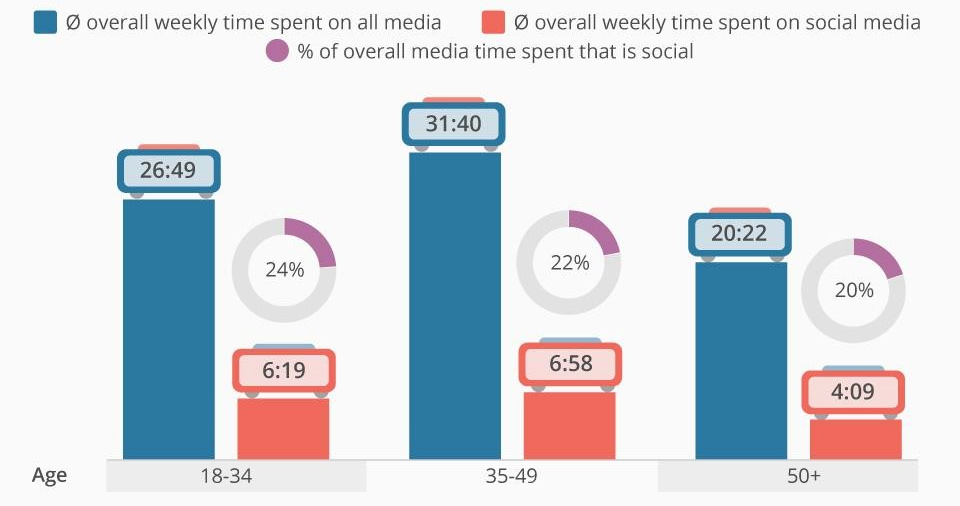
\includegraphics[width=.88\textwidth]{assets/gen-xy-time-spend-on-social-media.png}
    \caption[Porovnání času stráveného na sociálních sítích]{Porovnání času stráveného na sociálních sítích \\ Zdroj: The World Bank\protect\footnotemark }
    \label{fig:cas-na-socialnich-sitich}
\end{figure}

\footnotetext{Dostupné z: \url{http://web.worldbank.org/archive/website01603/WEB/MEDIA-31.HTM}}

Jak je vidět na obr. \ref{fig:cas-na-socialnich-sitich}, generace X tráví více času na médiích (včetně sociálních), než generace Y a to dokonce v řádu hodin. Toto lze vysvětlit např. způsobem, jakým mileniálové využívají svá mobilní zařízení. Analýzou více než 40 tisíc měsíčních účtů za telefon zjistila společnost Nielsen, že američtí teenageři odeslali v průměru \numprint{3146} textových zpráv za měsíc, což je asi 10 zpráv za hodinu v bdělém stavu a mimo školu.\cite[s. 33]{bergh2012coolznacky} Z dalšího výzkumu provedeného společností Deloitte\footnote{Dostupné z \url{https://blog.rescuetime.com/screen-time-stats-2018/}} vyplývá, že průměrně mileniálové kontrolují svůj telefon 58 krát za den, přičemž 70\rm \% těchto interakcí trvá méně než 2 minuty. Jiná studie dodává, že 1 z 10 teenagerů kontroluje svůj telefon alespoň jednou za 4 minuty\footnote{Dostupné z \url{https://nypost.com/2017/11/08/americans-check-their-phones-80-times-a-day-study}}.

Převedeno do marketingového kontextu, reklama cílená na generaci Y by měla být velmi krátká a měla by zaujmout okamžitě, jinak bude ignorována. Generace X bude klást větší důraz na její kvalitu a informační hodnotu.

Dále je velmi užitečné si uvědomit, jakou informační hodnotu médiím jednotlivé generace přidělují. Ve výzkumu provedeném společností eMarketer bylo zjištěno, že 82\rm \% věří tištěným reklamám nebo televizní či rádiové inzerci, zatímco pouhých 42\rm \% má důvěru ve výrobky či produkty, které jsou předmětem reklamy na sociální síti.\footnote{Dostupné z \url{https://www.emarketer.com/Article/Consumer-Trust-Evolving-Digital-Age/1014959}}


\section{Branding}
Moderní spotřebitelé jsou k novým či pro ně neznámým produktům skeptičtí a obvykle prvním krokem, než se rozhodnou pro koupi produktu, je vyhledání komentářů. Jak bylo podotknuto dříve v této práci, informace se v dnešní době šíří prakticky okamžitě a dohledat si je je velmi snadné. To dává do rukou spotřebitelů obrovskou moc a značky si tak musí být vědomy faktu, že i jedno potenciálně špatné hodnocení (byť neoprávněné) může odradit masu potenciálních zákazníků.
V průzkumu InSites Consulting zpracovali studii, ve které se dotazovaných ptali, který zdroj názorů je pro ně při rozhodování o koupi nových kusů oblečení nejdůvěryhodnější. Celkem 74\rm \% respondentů uvedlo, že je pro ně nejdůležitější názor jejich vrstevníků.\cite[s. 43]{bergh2012coolznacky}
Dalším negativním faktorem zejména pro mileniály pak může být neetické chování nebo špatný ekologický dopad. Mileniálové jsou uvědomělí spotřebitelé a problematika ochrany životního prostředí je stále palčivější. Demokratizaci zažívá ochrana planety obecně a pro generaci Y je typické, že se chce aktivně zapojovat a vytvářet vlastní hodnoty.

\subsection{Ztotožnění se se značkou}

Zatímco baby boomers generace si potrpěla na preciznost a kvalitu, pro generaci X a Y jsou mnohem důležitější hodnoty jako dobrá pověst (přitažlivost pro skupinu vrstevníků), kreativita a zábavnost a pravděpodobně nejdůležitější ze všech -- ztotožnění se se značkou. Značky a výrobky, které mladí kupují, se stávají jedním z ústředních bloků, s jejichž pomocí budují svou identitu. Vybírají si značky, se kterými se ztotožňují a které je charakterizují --- mileniálové obecně vykazují jisté formy narcismu, označovaného jako \uv{kampaň na sebe sama} --- a tím zboží dostává symbolickou hodnotu. Neslouží už jen jako nástroj a prostředek, ale zejména jako znak zastupující uvažování a hodnoty nositele.\cite{bergh2012coolznacky}

\subsection{Aakerův model}
Znalost značky sestává ze všech myšlenek, pocitů, představ, zkušeností, přesvědčení atd., které jsou spojovány se značkou. Značky musí u zákazníků především vytvářet silné, příznivé a jedinečné asociace.\cite[s. 315]{kotler2007marketingmanagement}
Příkladem může být společnost Volvo (bezbečnost), Hallmark (starostlivost), Apple (luxus).

Aaker, bývalý profesor marketingu na UC-Berkeley, pohlíží na hodnotu značky jako na soubor pěti kategorií aktiv a pasiv spojených se značkou\cite{kotler2007marketingmanagement}:
\begin{itemize}
    \item věrnost značce
    \item znalost značky
    \item vnímaná kvalita
    \item asociace spojované se značkou
    \item jiná duševní aktiva, např. patenty a obchodní známky
\end{itemize}

Jedinečný soubor asociací pak podle Aakera vytváří identitu značky sestávající se z 12 hledisek jak je ukazuje obr. \ref{fig:aaker-brand-identity-model}.

\medskip
\begin{figure}[htbp!]
    \centering
    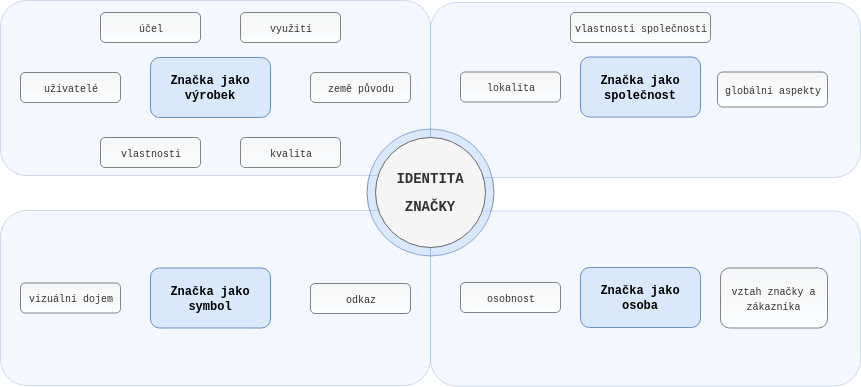
\includegraphics[width=.95\textwidth]{assets/aaker-model.png}
    \caption[Aakerův model identity značky]{Aakerův model identity značky \\ Zdroj: vlastní}
    \label{fig:aaker-brand-identity-model}
\end{figure}

\subsection{Loayalita ke značce}
% \include{chapters/04}
% \include{chapters/05}

\chapter*{Závěr}
\addcontentsline{toc}{chapter}{Závěr}

V úvodu této práce byl marketing prezentován jako umění i věda zároveň. Tato práce se soustřeďuje zejména na vědní část. Po teoretickém úvodu do marketingu jako takového prezentuje jednotlivé generace 20. a přelomu 21. století a pomocí shromážděných dat tyto generace charakterizuje z hlediska jejich priorit, sociálního chování a chování jako spotřebitelů.
Spotřebitele rozdělujeme podle doby, ve které vyrůstaly do tzv. \textit{generací}. Tyto generace jsou specifickými zákazníky. Každá vyrůstala v jiném režimu, měla k dispozici jiné prostředky. Konformistická \textit{tichá generace} se vyměnila za generaci \textit{baby boomers}, která se postavila proti režimu. Generace \textit{X} prožila ekonomickou recesi, aby ekonomiku připravila pro individualistické \textit{mileniály}. Marketing se musí vyvíjet spolu s generacemi a s technologickým pokrokem a k tomuto vývoji je důležitá znalost chování jednotlivých generací.\\
Cílem této práce bylo charakterizovat generace X a Y, tzv. mileniály z hlediska jejich chování jako spotřebitelů. Vzhledem k tomu, že tyto generace tvoří převážnou část současného trhu práce a generace mileniálů se má stát doposud nejpočetnější generací, je znalost jejich chování pro marketing velmi cenná. Tyto generace jsou si poměrně podobné, přesto je lze postavit v několika aspektech do kontrastu.
Generace X sledují aktuální technologické trendy a myslí dopředu, zdůrazňuje rovnováhu mezi soukromým a pracovním životem a je víc než kterákoli jiná ochotna slevit ze svých mzdových nároků za cenu flexibility pracovní doby. Naproti tomu mileniálové v technologii vyrůstaly a považují ji prakticky za samozřejmou, stejně tak považují za standard flexibilní pracovní dobu a z mzdových nároků slevují jen velmi těžko. Práce je pro ně brána jako součást života, proto takový důraz na rodinný život nekladou, za to vyzvihují individualitu a inkluzivní prostředí.\\
Aby byl marketing úspěšný, je potřeba jednotlivé rozdíly zmíněné v této práci brát v úvahu a stejně tak se adaptovat na podobnosti. Např., při tvorbě značky je důležité vytvořit, tzv. \uv{cool} značku, tj. značku, se kterou se generace ztotožňují, která v nich vzbuzuje emoce, pocit sounáležitosti, autenticity a luxusu. Při její propagaci pak vytvářet reklamu, která trvá pouze nezbytně dlouho a zaujme okamžitě, protože tyto mladé generace mají velmi rozdrobenou pozornost. Dle studijí prezentovaných v této práci je také užitečné zvolit vhodně sdělovací médium --- reklamy na sociálních sítích jsou pro generace X a Y nejen nedůvěryhodné, ale někdy dokonce označeny za obtěžující --- pro maximální efektivitu a maximalizaci zisku. Monogamní náklonnost je prakticky vyloučena, ale cool značky jsou konkurenceschopnější a zvyšují šanci, že si je zákazník zvolí jako svou první volbu.

%%% Seznam použité literatury
\printbibliography[title={Seznam použité literatury},heading={bibintoc}]


%%% Přílohy k bakalářské práci, existují-li. Každá příloha musí být alespoň jednou
%%% odkazována z vlastního textu práce. Přílohy se číslují.
% \part*{Přílohy}
% \appendix
% \include{app01}

\end{document}
